\documentclass[11pt]{beamer}
\usepackage[T1]{fontenc}
\usepackage[utf8]{inputenc}

\usepackage{pgf,pgfpages}

\usepackage{tikz}
\usetikzlibrary{arrows,shapes,backgrounds,calc}

\usepackage{graphicx}
\usepackage{colortbl}
\usepackage{units}

\usepackage{calrsfs}
% \DeclareMathAlphabet{\pazocal}{OMS}{zplm}{m}{n}
% \usepackage{calligra}
\usepackage[T1]{fontenc}

%% Beamer style >>>>>>>>>>>>>>>>>>>>>>>>>
\mode<presentation>
{
  \usetheme{PHD}
  \setbeamercovered{transparent}
  \setbeamertemplate{items}[square]
}

%\usefonttheme[onlymath]{serif}

\beamertemplatenavigationsymbolsempty

\defbeamertemplate{enumerate item}{mycircle}
{
  %\usebeamerfont*{item projected}%
  \usebeamercolor[bg]{item projected}%
  \begin{pgfpicture}{0ex}{0ex}{1.5ex}{0ex}
    \pgfcircle[fill]{\pgfpoint{-0.1pt}{.65ex}}{1.1ex}
    \pgfbox[center,base]{\color{PHDyellow}{\insertenumlabel}}
  \end{pgfpicture}%
}
[action]
{\setbeamerfont{item projected}{size=\scriptsize}}
\setbeamertemplate{enumerate item}[mycircle]

%<<<<<<<<<<<<< beamer style

\title[DG Approximations to Anisotropic Stokes]{Discontinuous Galerkin
  Approximation of Anisotropic Viscous Flows}
\author[J.R. Rodr\'{\i}guez Galv\'an]{\em J. Rafael Rodr\'{\i}guez
  Galv\'an\vspace{-0.9em}} \date{\footnotesize\structure{\em
    Doc-Course: ``Partial Differential Equations: Analysis, Numerics
    and Control''} \\[1ex] Granada. April 25, 2018}

% XeLaTeX font choosing
% \usepackage{fontspec}%{xltxtra} %fontspec}
% \setsansfont{Fontin Sans}
% \setsansfont{Lato}

% PDFLaTeX font choosing
\usepackage[default, scale=1.0]{lato}

\setbeameroption{hide notes} % Only slides
% \setbeameroption{show only notes} % Only notes
% \setbeameroption{show notes on second screen=right} % Both

% Different math fonts, see http://tug.org/pracjourn/2006-1/hartke/hartke.pdf
%\usepackage{eulervm}
%\usepackage{ccfonts, eulervm}
%\usepackage[math]{kurier}
%\usepackage[math]{anttor}
%\usepackage{pxfonts}
%\usepackage{mathpazo}
%\usepackage{mathpple}
%\usepackage[varg]{txfonts}
%\usepackage{arev}
%\usepackage{fourier}

\usepackage{tabularx}
\usepackage{array, multirow, booktabs, rotating} % booktabs: toprule, midrule...


\newcommand{\heatProblem}{(Heat-Problem)\xspace}
\newcommand{\poissonProblem}{(Poisson-Problem)\xspace}

% % Video playing
% % Commands with two or more optional arguments
% % (see http://tex.stackexchange.com/questions/29973/more-than-one-optional-argument-for-newcommand)
% \usepackage{xparse} % From future LaTeX 3
% \DeclareDocumentCommand{\PlayVideoWithLabelAutostart}{%
%   O{0.5\linewidth} O{0.5\linewidth}  O{} m }{%
%   % #1: width of video box
%   % #2: height of video box
%   % #3: Label
%   % #4: Video file
%   \begin{BoxWithVerticalLabel}{#3}{#1}
%     \href{run:#4?autostart}{\rule{#1}{#2}}
%   \end{BoxWithVerticalLabel}}

% \DeclareDocumentCommand{\PlayVideoWithNoLabelAutostart}{%
%   O{0.5\linewidth} O{0.5\linewidth} m }{%
%   \href{run:#3?autostart}{\rule{#1}{#2}}}

% \DeclareDocumentCommand{\PlayVideoNOAutoStart}{%
%   O{0.5\linewidth} O{1.0} O{} m }{%
%   \href{run:#3}{\rule{#1}{#2}}}

% \DeclareDocumentCommand{\PlayVideoWithLabelNOAutostart}{%
%   O{0.5\linewidth} O{1.0} O{} m }{%
%   \begin{BoxWithVerticalLabel}{#3}{#1}
%     \href{run:#4}{\rule{#1}{#2}}
%   \end{BoxWithVerticalLabel}}

% \DeclareDocumentCommand{\PlayVideoWithLabel}{%
%   O{0.5\linewidth} O{1.0}  O{} m }{\PlayVideoWithLabelAutostart[#1][#2][#3]{#4}}

% % \DeclareDocumentCommand{\PlayVideoWithLabel}{%
% %   O{0.5\linewidth} O{1.0}  O{} m }{\PlayVideoWithLabelNOAutostart[#1][#2][#3]{#4}}

\usepackage{presenta-granada-2018}

\newtheorem{remark}{Remark}
\newtheorem{proposition}{Proposition}
%\newtheorem{theorem}{Theorem}

% Presentation goodies >>>>>>>>>>>>>>>>>>>>>>>>>>>>
\newcommand<>{\myframed}[1]{\alt#2{\tikz[phd] \node[box] {#1};}{{#1}}}
\newcommand<>{\myframedAlert}[1]{\alt#2{\tikz[phdB] \node[boxB] {\color{black}#1};}{{#1}}}
\newcommand<>{\framedmath}[1]{%
\alt#2{\tikz[phd] \node[box] {\ensuremath{#1}};}{\ensuremath{#1}}}
\newcommand{\framedB}[1]{\tikz[phd] \node[boxB] {#1};}
\newcommand{\framedmathB}[1]{\framedB{\ensuremath{\displaystyle{#1}}}}
\newcommand{\ver}[1]{\footnote{See #1}}
\newcommand{\cita}[1]{{\color{PHDgray}\cite{#1}}}
\newcommand\cellalert[2]{\only<#1>{\cellcolor{PHDyellow}}\alt<#1>{\textbf{#2}}{#2}}
\newcommand{\soften}[1]{{\color{PHDgray}#1}}
\newcommand{\rowalert}[7]{%
    \cellalert{#1}{#2} & \cellalert{#1}{#3} &
    \cellalert{#1}{#4} & \cellalert{#1}{#5} &
    \cellalert{#1}{#6} & \cellalert{#1}{#7}}

\newcommand{\kk}{\Delta t}
% \usepackage{wasysym}
% \newcommand{\good}{{\color{PHDgreen}$\CIRCLE$}} %\blacksmiley
% \newcommand{\bad}{{\color{PHDred}$\CIRCLE$}}
\usepackage{pifont}
\newcommand{\good}{{\color{PHDgreen}\ding{52}}}
\newcommand{\bad}{{\color{PHDred}\ding{56}}}
\newcommand{\exclamation}{{\large\color{PHDred}{\textbf{\itshape !}}}}
\newcommand{\question}{{\large\color{PHDred}{\textbf{\itshape ?}}}}
\newcommand\colorUnderLine[2][PHDyellow]{\color{#1}\underline{{\color{black}#2}}\color{black}\xspace}
\newcommand\gris{\color{PHDgray}}
\newcommand\amarillo{\color{PHDyellow}}
\newcommand\tiragris[1]{{\par\hfill\small\gris{#1}}}
%<<<<<<<<<<<<<<<

\setcounter{tocdepth}{1}


%
% Bibliography
%
%\usepackage{natbib}

% To list each bibliographic entry in a line
\setbeamertemplate{bibliography entry title}{}
\setbeamertemplate{bibliography entry location}{}
\setbeamertemplate{bibliography entry note}{}

% ... end of preamble.

\AtBeginSection{\frame{\sectionpage}}


%======================================================================
\begin{document}
%======================================================================

% Tikz style and beamer template ------->>>
\tikzstyle{every picture}+=[remember picture]
\tikzstyle{na} = [baseline=-.5ex]
\tikzstyle{phd} = [baseline=-.6ex,
  box/.style={rectangle, draw=PHDblueC, thick, fill=PHDblueA,
    align=center, rounded corners, minimum height=1.6em},
  boxB/.style={rectangle, draw=PHDredA, thick, fill=PHDblueA,
    align=center, rounded corners, minimum height=1.6em}]
\tikzstyle{phdB} = [baseline=-.7ex,
  box/.style={rectangle, draw=PHDblueC, thick, fill=PHDblueA,
    align=center, rounded corners, minimum height=1.6em},
  boxB/.style={rectangle, draw=PHDredA, thick, fill=PHDblueA,
    align=center, rounded corners, minimum height=1.6em}]
\tikzstyle{myarrow} = [->,>=latex, PHDredA, shorten >=4pt,
  opacity=.6, line width=0.6mm]
\tikzstyle{myarrow2} = [->,>=latex, PHDblueC, shorten >=4pt, opacity=.2, line width=0.4mm]
\tikzstyle{myarrow3} = [
     opacity=.7,
%    >=triangle 60,              % Nice arrows; your taste may be different
    node distance=6mm and 60mm, % Global setup of box spacing
    every join/.style={norm},   % Default linetype for connecting
                                % boxes
    line width=0.6mm,
    PHDredA,
    ->
    ]
\setbeamertemplate{background}
 {
\includegraphics[width=\paperwidth,height=\paperheight]{frontpage_bg}}
\setbeamertemplate{footline}[default]
% <<<-------


% Write custom titlepage ------->>>
\begin{frame}
  \titlepage
  \vspace{5cm}
\end{frame}

% Set the background for the rest of the slides.
\setbeamertemplate{background}
 {
\includegraphics[width=\paperwidth,height=\paperheight]{slide_bg}}


% Write all of the slides..........

\begin{frame}{Outline}
  \tableofcontents
\end{frame}

% Start inserting infoline at the end
\setbeamertemplate{footline}[PHDtheme]
% <<<-------

\newcommand{\imgdir}{Undefined, use renewcommand!}

%============================================================================
\section{Preliminary Concepts and Notation}
%============================================================================


%---------------------------------------------------------------------
\begin{frame}{Distributional Derivatives}
%---------------------------------------------------------------------
  \begin{itemize}\itemsep0.9em
  \item
    $D(\Omega)= \big\{ \Phi\in C^\infty(\Omega) \text{ with compact
      support in } \Omega \big\}$
  \item $D'(\Omega)$ (dual space): space of \alert{distributions}
    \medskip
    \begin{itemize}
    \item Then $L^2(\Omega) \hookrightarrow D'(\Omega)$ \qquad
      ($v\in L^2(\Omega)\mapsto v(\Phi)=\int_\Omega v\phi$)
  \end{itemize}
\item \alert{Distributional derivative}: $\forall v\in D'(\Omega)$,
  $\forall\alpha=(\alpha_1,\dots,\alpha_d)\in\Nset^d$,
  $\partial^\alpha v \in D'(\Omega)$ is defined as:
    % $$\small
    % \langle \partial^\alpha v, \Phi \rangle_{D',D} = \partial^\alpha v(\Phi)
    % :=
    % \langle  v, (-1)^{|\alpha|}\partial^\alpha\Phi \rangle_{D',D} =
    % $$
    $$\small
    \partial^\alpha v(\Phi) := (-1)^{|\alpha|} v(\partial^\alpha\Phi), \quad \forall \Phi\in D(\Omega)
    $$
    \vspace{-1em}
    \begin{itemize}
    \item Then $\forall v\in L^2(\Omega)$ one has
      $\partial^\alpha v \in D'(\Omega)$ with:
    $$\small
    \partial^\alpha v(\Phi) = (-1)^{|\alpha|}\int_\Omega v \;
    \frac{\partial^{|\alpha|}\Phi}{\partial
      x_1^{\alpha_1}\dots\partial x_d^{\alpha_d}}
    \quad \forall \Phi\in D(\Omega)
    $$
  \end{itemize}
\end{itemize}
\end{frame}


\begin{frame}{Sobolev Spaces}
  \small
  \medskip
  $W^{s,p}(\Omega)=\big\{u\in D'(\Omega):\ \partial^\alpha u \in L^p(\Omega),\ |\alpha|\le s\big\}$
  \bigskip
\begin{itemize}\itemsep1em
\item Particular case \alert{$p=2$}:
  $$
  \alert{H^s(\Omega)}:=W^{s,\alert{2}}(\Omega)=\big\{u\in D'(\Omega):\
  \partial^\alpha u \in L^{\alert{2}}(\Omega),\ |\alpha|\le s\big\}
  $$
  \vspace{-1em}
  \begin{itemize}
  \item Hilbert space with scalar product and norm:
    $$
    (u, v)_s = \sum_{|\alpha|\le s}\int_\Omega \partial^\alpha u \partial^\alpha v,
    \qquad
    \norm[s]{u} = +\sqrt{ (u,u)_s }
  ~\vspace{-1em}~
    $$
  \end{itemize}
\item For instance,
  \begin{align*}
    \alert{H^0(\Omega)}&=L^2(\Omega), \quad (u,v)_0=(u,v)_{L^2(\Omega)}, \quad \norm[0]{u}=\norm[L^2(\Omega)]{u}
    \\[0.5em]
  \alert{H^1(\Omega)}&=\big\{u\in L^2(\Omega):\
  \partial_i u \in L^{{2}}(\Omega),\ 1\le i \le d\big\}
    \\
    &(u, v)_1 %= \int_\Omega u\,v + \sum_{i=1}^d \int_\Omega \partial_i u \partial_i v
    = \int_\Omega u\,v +  \int_\Omega \grad u \grad v
    \\
    &\norm[1]{u} = \left(\int_\Omega \norm[0]{u}^2 + \int_\Omega \norm[0]{\grad u}^2\right)^{1/2}
  \end{align*}

\end{itemize}
\end{frame}


\begin{frame}{Sobolev Embedding}
  \begin{theorem}
    For $\Omega\subset\Rset^d$, we have:
    $$
    H^s(\Omega)\subset C^r(\Omega) \quad \text{if}\quad \frac12 < \frac{s-r}d
    $$
  \end{theorem}
  In particular,
  $$
  H^s \subset C^0(\Omega) \quad \text{if}\quad
  \left\{
    \begin{aligned}
    s>\frac12 \quad \text{for}\quad d=1
    \\
    s> 1 \quad \text{for}\quad d=2
    \\
    s>\frac32 \quad \text{for}\quad d=3
  \end{aligned}
    \right.
  $$
% \begin{itemize}\itemsep1em
% \end{itemize}
  \small
  \color{gray}
  \textbf{Remark}:  Sobolev spaces with \textbf{fractional indices} $H^{s+1/2}(\Omega)$
  can be defined by interpolating between $H^s(\Omega)$ and $H^{s+1}(\Omega)$,
  so that they verify
  $$
  H^s(\Omega) \subset H^{s+1/2}(\Omega) \subset H^{s+1}(\Omega).
  $$
\end{frame}


\begin{frame}{Trace Theorems}
  % We define $H^1_0(\Omega)=\overline{D(\Omega)}^{H^1(\Omega)}$
% Using distributional derivatives, we can formulate partial differential equations in the dis-
% tributional sense. The notion of traces [81] is used to define the restriction of a Sobolev
% function along the boundary of the domain. This is important for properly defining boundary
% conditions.
  \begin{itemize}
  \item Let $\gamma_0:C^0(\overline\Omega)\to C^0(\partial\Omega)$, be
    the \alert{\bf trace} operator, \alert{$\gamma_0(v)=v|_{\partial\Omega}$}
  \item $\gamma_0$ can be continuously extended to $H^1(\Omega)$:
  \end{itemize}
  \begin{theorem}
    Let $\Omega$ be a Lipschitz open bounded set
    \begin{enumerate}
    \item The extended trace operator,
      $\gamma_0:H^1(\Omega)\to H^{1/2}(\partial\Omega)$ is
      surjective
    \item Moreover, the kernel of $\gamma_0$ is the set $H^1_0(\Omega)=\overline{D(\Omega)}^{H^1(\Omega)}$
    \end{enumerate}
  \end{theorem}
  \textbf{Remark}
  \begin{itemize}
  \item Statement (2) means that $H^1_0(\Omega)=\{ v \in H^1(\Omega):\ v=0\ \text{on}\ \partial\Omega\}$.
  \item Important trace inequalities that are frequently used in the analysis of
the DG methods: (...)
  \end{itemize}
\end{frame}


\begin{frame}{Meshes}
  Notation: \medskip
  \begin{itemize}\itemsep1em
  \item \structure{$\Th$}: \alert{mesh} of $\Omega$,
    $\Th = \{K_i\}_{i=1}^{N_t} \subset\Rset^d$ (``elements'' or
    ``triangles'')
    \medskip
    \begin{itemize}\itemsep0.4em
    \item $h_K:=\text{diam}(K)$, $h:=\max_{K\in\Th}(h_K)$
    \item Form simplicity, we consider \structure{conforming} meshes
      \structure{(not neccessary!)}
      \note[item]{\textbf{Conforming meshes}: For simplicity,
        we assume that the intersection of two elements is either empty, a
        vertex, an edge, or a face}
    \item Assume $\Th$ is \structure{regular}, ie:\vspace{-0.5em}
      $$\exists\rho:\quad \frac{h_K}{\rho_K} \le \rho
      \qquad  (\rho_K=\text{radius of ball in K} )
      $$
    \end{itemize}

  \item \structure{$\Eh$}: set of \alert{edges} ($d=2$) or faces ($d=3$)
    \llaveizq{\structure{$\Ehi$}: interior faces,\\[0.3em] \structure{$\Ehb$}: boundary faces}
    \begin{itemize}\itemsep0.5em

    \item We associate a unit normal vector $\nn_e$ to each edge $e$
    \item $h_e:=\text{diam}(e)$
    \item Relation: $\forall e\subset \partial K$, \quad
      \alert{$h_e \le C\; h_K^{d-1}$}
      \begin{flushright}\footnotesize
        \color{gray}due to regularity of $\Th$ and to the fact
          {$|e| \le h_K^{d-1}$},
          \\ $|e|:=$ length/area of edge/face $e$
      \end{flushright}
    \end{itemize}
  \end{itemize}
\end{frame}


\begin{frame}{Broken Sobolev Spaces}
\note[item]{Broken Sobolev spaces are natural spaces to work with the DG methods. These spaces
  depend strongly on the partition of the domain}
\begin{itemize}\itemsep0.7em
\item \textit{Broken} Sobolev space:
    \begin{equation*}
      \alert{H^m(\Th)} := \big\{ u\in L^2(\Omega) \ |\ u\in H^m(K),\ \forall K\in\Th \big\},
    \end{equation*}

    {\small Scalar product and norm:}\medskip
    \begin{itemize}\itemsep0.3em
    \item $\prodBroken[H^s(\Th)]{u,v }= \sum_{K\in\Th}\prodEsc[H^s(K)]{u,v}$
    \item $\normBroken[H^s(\Th)]{u}=\left(\sum_{K\in\Th}\norm[H^s(\Omega)]{u}^2 \right)^{1/2}$
    \end{itemize}

  \item Clearly, $H^m(\Omega)\subset H^m(\Th)$

  \item Particular  case: broken or \structure{discontinuous polynomials} spaces
    $$
    \alert{\Pd{k}(\Th)}=\left\{ v\in L^2(\Omega):\ v|_K\in \P{k}(K),\ \forall K\in\Th \right\}
    $$
  % \item Discontinous finite-dimensional subspace of $H^m(\Th)$:
  %   $$
  %   \structure{\Pd k(\Th)}:=
  %   \left\{
  %     u\in L^2(\Omega) \ | \ u\in \P{k}(K), \ \forall K\in\Th \right \}.
  %   $$
    \begin{flushright}
      \footnotesize
      \color{gray} Polinomials of degree at most $k$
    \end{flushright}
    \begin{itemize}
    \item Discontinuity along the \textbf{edges} (or faces)
    \end{itemize}
  \end{itemize}
\end{frame}

\begin{frame}{Jumps and averages}
  Let $\alert{v}\in H^m(\Th)$  \quad (\ $\Rightarrow$\ \alert{trace} of $v$ in any $K\in\Th$ is well defined\ )
  \bigskip
  \begin{itemize}\itemsep1em
  \item If $\alert{e}=K_1\cap K_2\in\Ehi$ is an \textbf{interior edge} \quad ($K_1,K_2\in\Th$)
    \medskip
    \begin{itemize}\itemsep0.7em
    \item Let $\alert{v|_{K_1}^e}$ and $\alert{v|_{K_2}^e}$ be
      the traces of $v$ along $e$. We define:
      \medskip
      \begin{itemize}\itemsep0.7em
      \item \alert{Jump}: $\structure{\jump{v}_e}:= v|_{K_1}^e-v|_{K_2}^e$
      \item \alert{Average}: $\structure{\average{v}_e} := \frac12 (v|_{K_1}^e+v|_{K_2}^e)$
      \end{itemize}
      \medskip
      % \begin{itemize}
      % \item[$\star$] If $e\in\Ehb$: $\jump{v}_e:= \average{v}_e:= v_e$
      % \end{itemize}
    \end{itemize}
  \item If $\alert{e}=K_1\cap \partial\Omega \in\Ehb$ is a \textbf{boundary edge} \quad ($K_1\in\Th$)
    \medskip
    \begin{itemize}\itemsep0.7em
    \item Let $\alert{v|_{K_1}^e}$ be the trace of $v$ along $e$. We
      just define: \medskip
      \begin{itemize}\itemsep0.7em
      \item \alert{Jump}: $\structure{\jump{v}_e}:= v|_{K_1}^e$
      \item \alert{Average}: $\structure{\average{v}_e} := v|_{K_1}^e$
      \end{itemize}
    \end{itemize}
  \end{itemize}
\end{frame}

\begin{frame}
    \begin{theorem}[Characterization of $H^1(\Omega)$]
      A function $v\in H^m(\Th)$ belongs to $H^1(\Omega)$ if and only if
      $$
      \jump{v}=0 \quad \forall e\in\Ehi
      $$
    \end{theorem}
\end{frame}
%============================================================================
\section{DG Formulation of Elliptic PDE}
%============================================================================
\label{sec:dg-elliptic-PDE}


%---------------------------------------------------------------------
\begin{frame}{Preliminary Concepts and Notation}
%---------------------------------------------------------------------
  \begin{itemize}
    \itemsep=0.95em
  \item \structure{$\Th$}: family of meshes of the domain $\Omega\subset\Rset^d$
  \item For instance, simplicial elements \structure{$K$} satisfying usual
    regularity:
    $$
    \exists \rho>0 \ /\ \rho\, h_K \le r_K \quad \forall K\in\Th,
    $$
  \item \structure{$\Eh$}: set of faces (edges in $2D$)\quad
    \llaveizq{\structure{$\Ehi$}: interior faces,\\[0.3em] \structure{$\Ehb$}: boundary faces}
  \item If $e=K^+\cap K^-\in\Ehi$ \llaveizq{jump: $\structure{\jump{u}_e}:= u|_{K^+}-u|_{K^-}$, \\[0.4em]
   mean: $\structure{\average{u}_e} := \frac12 (u|_{K^+}+u|_{K^-})$}
 \medskip
 \begin{itemize}
 \item[$\star$] If $e\in\Ehb$: $\jump{u}_e:= \average{u}_e:= u_e$
 \end{itemize}
\end{itemize}
\end{frame}

%---------------------------------------------------------------------
\begin{frame}{Notation II}
%---------------------------------------------------------------------
  \begin{itemize}
    \itemsep=0.95em
  \item \textit{Broken} Sobolev space:
    \begin{equation*}
      \structure{H^m(\Th)} := \big\{ u\in L^2(\Omega) \ |\ u\in H^m(K)\ \forall K\in\Th \big\},
    \end{equation*}
  \item Broken gradient operator \structure{$\gradh$}:
    $\forall u\in H^1(\Th)$,
    $$
    (\gradh u)|_K=\grad(u|_K)\quad \forall\, K\in\Th
    $$
  \item Discontinous finite-dimensional subspace of $H^m(\Th)$:
    $$
    \structure{\Pd k(\Th)}:=
    \left\{
      u\in L^2(\Omega) \ | \ u\in \P{k}(K), \ \forall K\in\Th \right \}.
    $$
    \begin{flushright}
      \footnotesize
      \color{gray} Polinomials of degree at most $k$
    \end{flushright}
    \begin{itemize}
    \item Test functions are \textbf{discontinuous} along the \textbf{edges} (or faces)
    \end{itemize}
  %   $$
  %   \structure{\Qd k(\Th)}:=
  %   \left\{
  %     u\in L^2(\Omega) \ | \ u\in \Q{k}(K), \ \forall K\in\Th \right \}.
  %   $$
  %   \begin{flushright}
  %     \footnotesize
  %     \color{gray} Polinomials of degree at most $k$ in each variable
  %   \end{flushright}
  \end{itemize}
\end{frame}

%---------------------------------------------------------------------
\begin{frame}{SIP (Symmetric Interior Penalty) Bilinear Form}
% ---------------------------------------------------------------------
  \textbf{\itshape Poisson problem} (homogeneous Dirichlet b.c.)
  % \vspace{-1em}
  \begin{center}
    + integration by parts in each element
    \small\cite{arnold_interior_1982,di_pietro_ern_2012}
    \quad
    $\leadsto$
  \end{center}
  \vspace{-1em}
  \begin{multline*}
    \asip[sip,\alert<3>{\eta}](\uh,\buh) = \int_\Omega \gradh \uh \cdot\gradh\buh
    \\
    \framedmath<2>{\displaystyle - \sum_{e\in\Eh} \int_e\big( \average{\gradh \uh}\cdot \nn_e \jump{\buh}
      + \jump{\uh} \average{\gradh\buh}\cdot \nn_e \big)
    }
    \\
    + \framedmath<3>{\displaystyle\alert<3>{\mathbf{\eta}}\sum_{e\in\Eh} \frac1{h_e} \int_e \jump{\uh}\jump{\buh}},
    \quad \forall\,\uh,\buh\in \Pd k
  \end{multline*}
  \vspace{-1em}
  \begin{itemize}
  \item<2> \myframed{Consistency and symmetry}
  \item<3> \myframed{Coercivity (for $\alert<3>{\mathbf{\eta}>0}$ big enough)}
  \end{itemize}
\end{frame}

%---------------------------------------------------------------------
\begin{frame}{SIP (Symmetric Interior Penalty) Bilinear Form II}
  % ---------------------------------------------------------------------
  \begin{definition}[SIP norm]
    \begin{equation*}
      \normsip{u} = \big(\, \norm[]{\gradh u}^2 + \seminormU{u}^2 \;\big) ^{1/2},
    \end{equation*}
    where
    \begin{equation*}
      \seminormU{u} =
      \Big (\sum_{e\in\Eh} \frac1{h_e} \int_e {\jump u}^2 \Big ) ^{1/2} \quad \text{(\textit{jump seminorm})}.
    \end{equation*}
  \end{definition}
  \begin{lemma}[Coercivity and Continuity]
    \begin{itemize}
    \item Exists $C(\eta)>0$ such that
      \begin{equation*}
        \asip[sip,\eta](\uh,\uh) \ge C(\eta) \normsip{\uh}^2, \quad \forall\,\uh\in \Pd k
      \end{equation*}
    \item Exists $ C_{\text{bnd}}>0$ such that
      \begin{equation*}
        \label{eq:sip:boundedness}
        \asip[sip,\eta](\uh,\buh) \le C_{\text{bnd}} \normsip{\uh}\normsip{\buh}, \quad \forall\,\uh,\buh\in \Pd k
      \end{equation*}
    \end{itemize}
  \end{lemma}
  \begin{flushright}
    \scriptsize \textbf{Proof}: see e.g.\cite{di_pietro_ern_2012}
  \end{flushright}
\end{frame}

% %%,---------------------------------------------------------------------
% %%|
% %%`---------------------------------------------------------------------
%============================================================================
% \section[Introduction]{Stability of Anisotropic Stokes Equations}
%============================================================================
% \label{sec:introduction}

% \begin{frame}{Anisotropic equations for (large scale) ocean}
% %----------------------------------------------------------------------
%   \begin{itemize}\itemsep0.5em
%   \item<1> \structure{The ocean:} A slightly compressible fluid
%     endowed with Coriolis and buoyancy forces and a set of
%     conservation laws from
%     Physics
%   \item<2-> Simplification of physical laws:\vspace{-1em}
%     \begin{columns}
%       \column{0.05\linewidth}
%       \column{0.41\linewidth}
%       \begin{enumerate}\itemsep1.5em
%       \item<2-> Boussinesq hypothesis
%         \tikz[na] \coordinate(Lboussinesq);
%         \hfill
%         \tikz[na] \coordinate(Rboussinesq);
%       \item<3-> Cartesian coordinates
%         \tikz[na] \coordinate(LbetaPlane);
%         \hfill
%         \tikz[na] \coordinate(RbetaPlane);
%       \item<4-> Vertical scaling
%         \tikz[na] \coordinate(LverticalScaling);
%         \hfill
%         \tikz[na] \coordinate(RverticalScaling);
%       \end{enumerate}
%       \column{0.54\linewidth}
%       \begin{overprint}
%         \onslide<2>
%         \begin{block}{Boussinesq Hypothesis}
%           \begin{itemize}
%           \item \textit{Density} does not depart from a \textit{mean reference value},
%             $\rho_\star>0$
%           \item Hence density can be replaced by the constant
%             $\rho_\star$ except in
%             % \begin{itemize}
%             % \item
%               \textit{buoyancy} term
%             % \item conservation of \textit{energy equation}
%               {\color{PHDgrayC} (and state equation)}
%           \end{itemize}
%         \end{block}
%         \onslide<3>
%         \begin{block}{Cartesian Coordinates}
%           \begin{itemize}
%           \item A \textit{local projection} of the Earth surface will be
%             assumed
%           \item \textit{No loss of generality}: spherical coordinates requires
%             only the proper handling of some terms
%           \end{itemize}
%         \end{block}
%         \onslide<4>
%         \begin{block}{Vertical Scaling of Domain}
%           \vspace{-0.5em}
%           \begin{itemize}
%           \item The \textit{aspect ratio}
%             \begin{equation*}
%               \framedmath{\displaystyle\varepsilon = \frac{\text{vertical
%                     scales}}{\text{horizontal scales}}}~
%                 \begin{tabular}[t]{l} is \large\textbf{small} \\[-0.2ex]
%                   \tiny\it ~ $10^{-3}$, $10^{-4}$\end{tabular}
%             \end{equation*}
% %            \pause
%           \item \scriptsize \emph{Physical} point of view: dominant terms in
%             \textit{vertical momentum} equation
%           \item \emph{Numerical} point of view: the problem is
%             \textit{rescaled}, obtaining...
%             \begin{itemize}
%             \item \alert{\textbf{Isotropic domain}}
%             \item \alert{\textbf{Anisotropic equations}}
%             \end{itemize}
%           \end{itemize}
%         \end{block}
%       \end{overprint}
%     \end{columns}
%   \end{itemize}
% \end{frame}

% %----------------------------------------------------------------------
% \begin{frame}{Isotropic domain}
% %----------------------------------------------------------------------
% %  \vspace*{0.5em}
%  After geometrical scaling, we obtain:
%    $$
%    \domain = \bigl\{ (\xx,z)\in \Rset^{3} \ /\ \xx=(x,y)\in\surface,\
%    -D(\xx)< z < 0 \bigr\},
%    $$
%    where $\surface\subset\Rset^{2}$ is surface domain and
%    $D:\overline\surface \to \Rset_{+}$ is depth function
%    \begin{center}
%      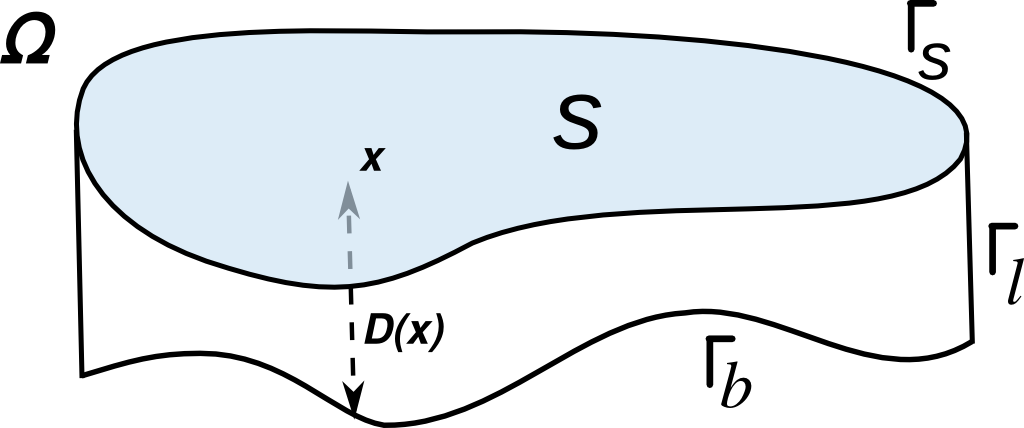
\includegraphics[width=0.4\textwidth]{img/domain}
%    \end{center}
%    \begin{itemize}
%      \setlength\itemsep{1em}
%    \item \alert{Rigid lid hypothesis} (flat surface) is introduced
%    \item
%      \color{darkgray} Notation:
%      \begin{itemize}
%      \item \color{darkgray} $\surfaceBoundary$: part of the boundary corresponding to
%        the surface
%      \item \color{darkgray} $\bottomBoundary$: part corresponding to the bottom
%        boundary
%      \item \color{darkgray} $\talusBoundary$: lateral walls (if any)
%      \end{itemize}
%    \end{itemize}
%  \end{frame}

% %----------------------------------------------------------------------
% \begin{frame}{Anisotropic equations}
% %----------------------------------------------------------------------
% %  \vspace{-0.2em}
%   \note{Comment briefly the main difficulties of Navier-Stokes equations}
%   \begin{overprint}
%     \onslide<1>
%     Anisotropic momentum equations (in the isotropic) domain:
%     \onslide<2>
%     \alert{Vertical/Horizontal aspect ratio} \tikz[na] \coordinate(LaspectRatio);
%     \  affects vertical velocity terms!
%     \onslide<3>
%     \alert{Coriolis} force
%     \tikz[na] \coordinate(Lcoriolis);
%     \onslide<4>
%     \alert{\textbf{Density}}: \textbf{coupling} of energy equations.
%     \tikz[na] \coordinate(Lcoupling);
%     \onslide<5>
%     \textbf{We focus on \dotfill \alert{Constant density case}}
%     \onslide<6>
%     \textbf{We focus on \dotfill \alert{Linear steady case}}
%   \end{overprint}
%   \begin{block}{\small Conservation of momentum and continuity}
%     \vspace{-0.66\baselineskip}
%     \begin{align*}
%       {\onslide<1-5> \dt \uu + \uu\cdot\gradx\uu + \vv\,\dz\uu  {\onslide<-6>- \visc\Delta\uu
%       +}} {\onslide<1-4>\frac 1 \rho_\star} \onslide<-6> \gradx \pp=
%        \tikz[na] \node (Rcoriolis) {\framedmath<3>{\fU}};
%       \\
%       \tikz[na] \coordinate(RaspectRatio);
%         \framedmath<2>{ \varepsilon^2 \Big( {\onslide<1-5> \dt \vv + \uu\cdot\gradx\vv +
%           \vv\,\dz\vv} {\onslide<-6> - \visc\Delta\vv \Big) }}
%         \displaystyle
%         + {\onslide<1-4> \frac 1 \rho_\star } {\onslide<-6> \dz \pp} +
%         {\onslide<1-4> \frac{1}{\rho_\star}} \tikz[na] \coordinate(RcouplingA);
%           \framedmath<4>{\rho}\,\gravity {\onslide<-6> = 0\hskip+0.5em}
%       \\[-0.2em]
%       \div\uu + \dz\vv = 0\hskip+0.5em
%     \end{align*}
%     \vspace{-1.4\baselineskip}
%   \end{block}
%   \begin{block}<4>{\small Convection-diffusion of \textit{temperature} and
%       \textit{salinity} + state equation (density)}
%     \vspace{-0.66\baselineskip}
%     \begin{align*}
%       \dt \Te  + (\uu \cdot \gradx) \Te + (\vv\cdot\dz) \Te  - \nu_\Te\Delta \Te &= \fT
%       \\[0.3em]
%       \dt \Sa  + (\uu \cdot \gradx) \Sa + (\vv\cdot\dz) \Sa -
%       \nu_\Sa\Delta \Sa &= \fS
%       \\[0.3em]
%       \tikz[na] \coordinate(RcouplingB);
%       \framedmath<4>{\rho} = \rho_\star\big(1-\beta_\Te(\Te-\Te_\star) + \beta_\Sa(\Sa&-\Sa_\star)\big)
%     \end{align*}
%     \vspace{-1.4\baselineskip}
%   % \item Equation of state (dependence of density in terms of
%   %   temperature and salinity)
%   %   where $\Te_\star$ and $\Sa_\star$ are given reference values.
%   \end{block}
%   \tikzstyle{RaspectRatio} = [draw, circle, minimum size=.5cm, node
%   distance=1.75cm]
%   \tikzstyle{redcircle} = [draw, circle, color=PHDredA, node distance=3cm,
%   minimum height=2em]

%   \begin{tikzpicture}[overlay]
%     \path<2>[myarrow]
%     (LaspectRatio) edge [out=320, in=130] (RaspectRatio);
%     \path<3>[myarrow]
%     (Lcoriolis) edge [out=0, in=130] (Rcoriolis);
%     \path<4>[myarrow]
%     (Lcoupling) edge [out=0, in=135] (RcouplingA);
%     \path<4>[myarrow]
%     (Lcoupling) edge [out=0, in=135] (RcouplingB);
%         % \draw<3>[->, PHDblue, ultra thick, opacity=.8] (Lboussinesq) -- (Rboussinesq);
%         % \draw<4>[->, PHDblue, ultra thick, opacity=.8] (LbetaPlane) -- (RbetaPlane);
%         % \draw<5>[->, PHDblue, ultra thick, opacity=.8] (LverticalScaling) -- (RverticalScaling);
%   \end{tikzpicture}
% \end{frame}

% %--------------------------------------------------------------------------
% \begin{frame}{Steady Anisotropic Stokes equations}
% %--------------------------------------------------------------------------
%   \color{darkgray}{\small Thus we are interested in numerical resolution of:}
%   \bigskip
%   \begin{center}\large
%     \textit{mixed anisotropic velocity/pressure problems}
%   \end{center}
%   \bigskip
%   \begin{center}
%     \uncover<2>{... when $\framedmath<2>{\varepsilon\to 0}$}
%   \end{center}
%   \begin{block}{Steady Anisotropic Stokes equations}
%     \begin{equation*}
%       \begin{aligned}
%         - \nu\Delta\uu + \gradx\pp &= \ff,
%         \\
%         \framedmath<2>{-\varepsilon^2 \Delta\vv} + \dz\pp &= 0,
%         \\
%         \divx\uu + \dz\vv &= 0.
%       \end{aligned}
%     \end{equation*}
%   \end{block}
% \end{frame}


% %--------------------------------------------------------------------------
% \begin{frame}{Not Easy Task!}
% %--------------------------------------------------------------------------
%   \begin{center}
%       \begin{tabular}[b]{r}
%         $\P2/\P1$ F.E.
%         \\[1ex]
%         Velocity
%         \\[1ex]
%         \alert{$\framedmath{\varepsilon=10^{-2}}$}
%         \\
%         \rule{0pt}{0.5\textheight}
%       \end{tabular}
%       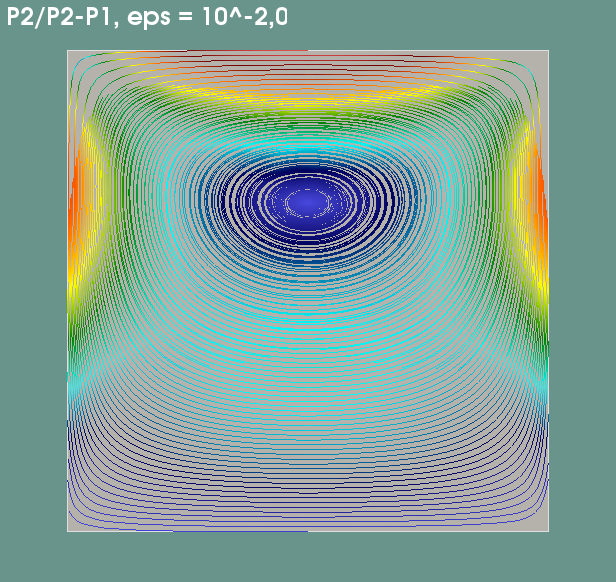
\includegraphics[width=0.7\linewidth]{img/221-eps-2}
%   \end{center}
% \end{frame}

% %--------------------------------------------------------------------------
% \begin{frame}{Not Easy Task!}
% %--------------------------------------------------------------------------
%   \begin{center}
%       \begin{tabular}[b]{r}
%         $\P2/\P1$ F.E.
%         \\[1ex]
%         Velocity
%         \\[1ex]
%         \alert{$\framedmath{\varepsilon=10^{-3}}$}
%         \\
%         \rule{0pt}{0.5\textheight}
%       \end{tabular}
%       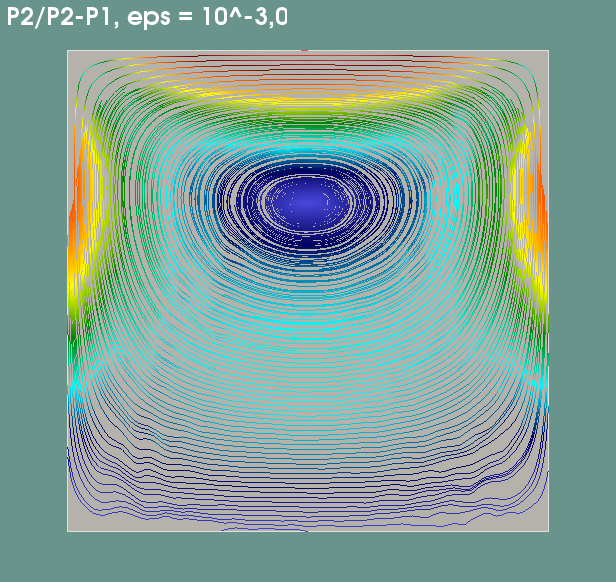
\includegraphics[width=0.7\linewidth]{img/221-eps-3}
%   \end{center}
% \end{frame}

% %--------------------------------------------------------------------------
% \begin{frame}{Not Easy Task!}
% %--------------------------------------------------------------------------
%   \begin{center}
%       \begin{tabular}[b]{r}
%         $\P2/\P1$ F.E.
%         \\[1ex]
%         Velocity
%         \\[1ex]
%         \alert{$\framedmath{\varepsilon=10^{-4}}$}
%         \\
%         \rule{0pt}{0.5\textheight}
%       \end{tabular}
%       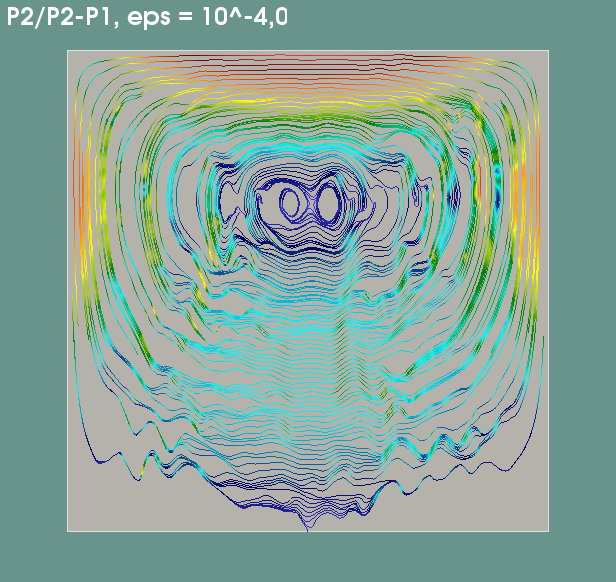
\includegraphics[width=0.7\linewidth]{img/221-eps-4}
%   \end{center}
% \end{frame}

% %--------------------------------------------------------------------------
% \begin{frame}{Instability of \textit{Classical} Finite Elements}
% %--------------------------------------------------------------------------
%   \begin{itemize}
%     \itemsep=1.2em
%   \item ``Classical'' Taylor-Hood $\P2/\P1$ F.E. \textbf{not stable} when $\varepsilon\to 0$
%   \item Similar results for bubble $\P{1,b}/\P1$ F.E.
%   \item Why? \ \ One has stokes-like inf-sup condition...
%     \par\hfill\uncover<2->{\alert<2>{and also a \textbf{new hydrostatic inf-sup condition}}}
%     \begin{alignat*}{4}
%       \label{eq:ISp}
%       \tag*{\ensuremath{(IS)^\PP}\xspace}
%       &\quad&
%       \sup_{0\neq(\uu,\vv)\in \UU \times \VV}
%       \frac{(\div(\uu,\vv),\pp)}{\|\grad \uu,\dz \vv\|}
%       &\ge \ConstISp \|\pp\|
%       &\quad&
%       \forall \pp \in \PP,
%       \\[1.0em]
%       \label{eq:ISv}
%       \onslide<2->
%       \tag*{\ensuremath{(IS)^\VV}\xspace}
%       &\quad &
%       \alert<2>{
%         \sup_{0\neq \pp \in \PP}
%         \frac{(\dz \vv,\pp)}{\|\pp\|}}
%       &\alert<2>{\ge \ConstISv \|\dz\vv\|}
%       &\quad&
%       \alert<2>{\forall \vv\in \VV}
%     \end{alignat*}
%   \item<3> New inf-sup condition means:
%     \begin{center}
%       \structure{\# dofs($\alert{v}$)} not bigger than \structure{\#
%         dofs($\alert{p}$)}
%     \end{center}
%   \end{itemize}
% \end{frame}

% %---------------------------------------------------------------------
% \begin{frame}{How to proceed?}
% %---------------------------------------------------------------------
%   \begin{description}
%     \itemsep=1.5em
%   \item[Idea 1] To introduce \textbf{new \emph{anisotropic} F.E.}~\cite{fguillen-rrgalvan-paper2-NumMath:2015,fguillen-rrgalvan-paper1-ApNumMath:2016}
%     \begin{flushright}\it
%       (which verify~\ref{eq:ISp} and also~\ref{eq:ISv})
%     \end{flushright}
%   \item[Idea 2] To introduce \textbf{new \emph{stabilized} schemes}~\cite{fguillen-rrgalvan-paper3-SIAM:2015}
%     \begin{flushright}\it
%       (which do not require~\ref{eq:ISv})
%     \end{flushright}
%   \item<2>[Idea 3] To \myframed{\textbf{Explore Discontinuous Galerkin F.E.}}
%     \begin{flushright}\it
%       (which, in some sense, verify~\ref{eq:ISp} and also~\ref{eq:ISv})
%     \end{flushright}
%   \end{description}
% \end{frame}



%============================================================================
% \section[DG Formulation]{SIP DG Formulation for Anisotropic Stokes}
%============================================================================
% \label{sec:Stokes-dg-formulation}

% %---------------------------------------------------------------------
% \begin{frame}{DG Bilinear Form for Anisotropic Stokes}
% % ---------------------------------------------------------------------
%   \medskip
%   \small
%   % \begin{itemize}
%     % \itemsep=1em
%   % \item
%   \structure{\bf Order \underline{$k$} polynomials for \underline{\textit{velocity}} and \underline{\textit{pressure}}}: \llaveizq{$\wwh=(\uuh,v_h)\in\WWh$, \\
%     $\ph \in \Ph$,}
%     \begin{align*}
%       \WWh&=\UUh\times\Vh=(\Pd k)^d, \quad \UUh = (\Pd k)^{d-1}, \quad \Vh=\Pd k
%       \\
%       \Ph &= \Pd k.
%     \end{align*}
%     % For each $\wwh=(\uuh,\vh)$ and $\bwwh=(\buuh,\bvh) \in\WWh$, with
%     % $\uuh=(u_i)_{i=1}^{d-1}$ and $\buuh=(\overline u_i)_{i=1}^{d-1}$,
%   % \item
%     \medskip
%     \structure{\bf Anisotropic velocity bilinear form}: \enspace
%     $\forall \wwh=(\uuh,\vh),\ \bwwh=(\buuh,\bvh) \in\WWh$,
%     \begin{equation*}
%       a_h(\wwh,\bwwh) = \Big( \sum_{i=1}^{d-1} \asip[sip , \eta](u_i,\overline u_i)
%       + \tikz[na] \node(Laepsilon){\framedmath<2>{\alert<2>{\asip[\varepsilon](\vh,\bvh)}}};
%       \Big),
%     \end{equation*}
%     \vspace{-0.5em}
%     \onslide<2>
%     where
%     \begin{multline*}
%       \alert{\framedmath<2>{\asip[\varepsilon](\vh,\bvh)} =\tikz[na] \coordinate (Raepsilon);}
%       \\
%       \alert{ \varepsilon \,\asip[sip, 0](\vh,\bvh)
%       + \eta\sum_{e\in\Eh} \frac1{h_e} \int_e \Big( \varepsilon
%       \jump{\vh\nx}\jump{\bvh\nx} + \jump{\vh\nz}\jump{\bvh\nz} \Big),}
%     \end{multline*}
%     \begin{itemize}
%     \item[$\star$] \scriptsize $\varepsilon$--dependent bilinear form,
%       standard $\vh$ SIP stabilizing term is replaced by anisotropic term
%     \item[$\star$] Generalization of previous works (for Isotropic \&
%       Hydrostatic viscous
%       fluids~\cite{Guillen-RedondoNeble-RGalvan:17})
%     \end{itemize}
%   \begin{tikzpicture}[overlay]
%     \path<2>[myarrow] (Laepsilon) edge [out=210, in=40] (Raepsilon);
%   \end{tikzpicture}
% \end{frame}

% %---------------------------------------------------------------------
% \begin{frame}{Partial $\varepsilon$--dependent Coercivity}
% % ---------------------------------------------------------------------
%   \begin{itemize}
%     \itemsep=1em
%   \item For \underline{$\uuh$}, coercivity of SIP bilinear form yields:
%     \begin{equation*}
%       \sum_{i=1}^{d-1} \asip[sip , \eta](u_i,\overline u_i) \ge
%       C(\eta) \normsip{\uuh}^2 \quad
%       \structure{\scriptsize=\quad C(\eta) \sum_{i=1}^{d-1}\normsip{u_i}^2}
%     \end{equation*}
%   \item
%     For \underline{$(\uuh,\vh)$} we can show:
%     \begin{lemma}[$\varepsilon$--dependent coercivity]
%       For all $\eta>\eta_*$ and for all $\wwh=(\uuh,\vh) \in \WWh$,
%       \begin{equation*}
%         a_h(\wwh,\wwh) \ge C(\eta) \Big(
%         \normsip{\uuh}^2
%         + \varepsilon  \norm[0]{\gradh\vh}^2
%         % + C_{\eta}^{\varepsilon}\seminormVeps{\vh}^2
%         + \seminormVeps{\vh}^2
%         \Big),
%       \end{equation*}
%       where
%       $$
%       \seminormVeps{\vh}^2 = \sum_{e\in\Eh} \frac1{h_e} \int_e\Big(
%       \varepsilon\jump{\vh\nx}^2 + \jump{\vh \nz}^2 \Big).
%       $$
% \end{lemma}
% \end{itemize}
% \begin{scriptsize}
% \hfill \textit{Proof}:
%   (1) write $\asip[\varepsilon](\vh,\bvh)$ in terms of
%     $\varepsilon\asip[sip , \eta](\vh,\bvh)$,\enspace (2) apply coercivity of $\asip[sip , \eta](\vh,\bvh)$
% \end{scriptsize}
% \end{frame}

% %---------------------------------------------------------------------
% \begin{frame}{Partial $\varepsilon$--dependent Coercivity II}
% % ---------------------------------------------------------------------
%   \begin{itemize}
%     \itemsep=0.75em
%   \item The norm used in previous Lemma degenerates when $\varepsilon\to 0$
%   \item We redefine it, introducing $\framedmath{\dzh\vh}$:
%     \begin{align*}
%       \alert{\normsip{\vh}{_{,\varepsilon}}}= \left( \varepsilon\norm[0]{\gradxh\vh}^2 + \framedmath{\norm[0]{\dzh\vh}^2} +
%       \seminormVeps{\vh}^2\right)^{1/2},
%       \\[0.5em]
%       \text{and consider}\enspace \normveleps{\wwh} = \left(\normsip{\uuh}^2 + \alert{\normsip{\vh}}^2{_{,\varepsilon}}\right)^{1/2}.
%     \end{align*}
%   \item And we have an \textit{hydrostatic} inf-sup condition for $\framedmath{\dzh\vh}$:
% \begin{lemma} [Inf-Sup stability for $\dzh\vh$]
%   \begin{equation}
%     \tag*{\ensuremath{(IS)^\Vh}\xspace}
%     \norm[0]{\dzh\vh} =
%     \sup_{\bph \in \Ph}\frac{\int_{\Omega} \bph \, \partial_{z,h}\,\vh}{\|\bph\|_{0}}
%     \quad \forall\vh\in\Vh.
%   \end{equation}
%   \label{lemma:vh.stability}
% \end{lemma}
%   \end{itemize}
% \end{frame}

% %% ,---------------------------------------------------------------------
% %%| Conclusions and future work
% %%`---------------------------------------------------------------------
% \begin{frame}{Conclusions}
%   \begin{itemize}\itemsep0.66em
%   \item<1-> We have developed \alert{new schemes} for approximation of
%     Primitive Equations of the Ocean (or even Anisotropic Navier-Stokes)
%     \begin{itemize}
%     \item Avoiding velocity instabilities of (quasi-)hydrostatic
%       formulations
%     \end{itemize}
%   \item<2-> \alert{Standard FE tools and techniques} like mesh adaptation
%     can be used, in \alert{more general meshes} than previous schemes
%   \item<3-> Two different approached have been followed:
%     \begin{itemize}
%     \item New \alert{stable combinations of FE} (unequal
%       approximation of velocity components)
%     \item Reformulation of space schemes, \alert{stabilizing vertical
%       velocity}. Hence standard Stokes--stable FE can be applied
%     \end{itemize}
%   \item<4-> Successfully applied to \alert{time-dependent problems},
%     including \alert{variable density}
%   \end{itemize}
%   \uncover<5>{
%   \begin{center}\it
%     {In short, we have successfully introduced \textbf{a new approach}\\
%     for modelling \textbf{realistic hydrostatic and quasi-hydrostatic fluids},\\
%     justifying it both \textbf{analytically and numerically}.
%   }
% \end{center}
% }

% \end{frame}
% \begin{frame}{~}
%   \bigskip
%   \Large Thank you for your attention.
%   \vfill~
%   \begin{flushright}
%     \pgfsetfillopacity{0.4}
%     \pgfimage[width=0.9\textwidth]{img/gibraltar-velocity-2d-difumin}
%   \end{flushright}
% \end{frame}

%%,-------------
%%| Bibliography
%%`-------------

\setbeamertemplate{footline}[default]

\begin{frame}[allowframebreaks]{Bibliography}
\bibliographystyle{alpha}
%\bibliographystyle{abbrvnat}
\bibliography{biblio-short.bib}
\end{frame}

\end{document}


%%% Local Variables:
%%% coding: utf-8
%%% TeX-master: t
%%% mode: latex
%%% ispell-local-dictionary: "english"
%%% End:
